\documentclass[a4paper, 12pt]{article}
\usepackage[english]{babel}
\usepackage[utf8]{inputenc}
\usepackage[T1]{fontenc}
\usepackage{lmodern}
\usepackage{hyperref}
\usepackage[numbers, sort&compress]{natbib}
\usepackage{calc}
\usepackage{fancyhdr}
\usepackage{graphics}
\usepackage{nowidow}
\usepackage{color}
\usepackage{subcaption}
\usepackage{epsfig}
\usepackage{epstopdf}
\usepackage{verbatim}


\newlength{\oneLine}
\newlength{\halfLine}
\setlength{\oneLine}{12pt}
\setlength{\halfLine}{6pt}

\newlength{\eqMargin}
\newlength{\eqHorizMargin}
\newlength{\eqVertMargin}

\setlength{\eqMargin}{20mm}
\setlength{\eqHorizMargin}{\eqMargin}
\setlength{\eqVertMargin}{\eqMargin}

% Paper
\setlength{\paperwidth}{210mm}
\setlength{\paperheight}{297mm}

% Rid the extra space
\setlength{\hoffset}{-1in}
\setlength{\voffset}{-1in}
\addtolength{\hoffset}{\eqHorizMargin}
\addtolength{\voffset}{\eqVertMargin}

% Set margin from the page border (horizontal)
\setlength{\oddsidemargin}{0pt}
\setlength{\evensidemargin}{0pt}

% Header
\setlength{\topmargin}{0pt}
\setlength{\headheight}{42pt}
\setlength{\headsep}{18pt}
\renewcommand{\headrulewidth}{0pt}

% Footer
\addtolength{\footskip}{18pt}
\renewcommand{\footrulewidth}{0pt}

% Margin notes
\setlength{\marginparsep}{0pt}
\setlength{\marginparwidth}{0pt}

% Text
\setlength{\textwidth}{\paperwidth - \hoffset - \hoffset - 25.4mm - 25.4mm}
\setlength{\textheight}{\paperheight - \voffset - \topmargin - \headheight - \headsep - \footskip - \voffset - 25.4mm - 25.4mm}

%\setlength{\labelwidth}{20mm}

% Hyperref settings
\hypersetup{
    unicode=true,					% non-Latin characters in Acrobat's bookmarks
    pdftoolbar=true,				% show Acrobat's toolbar?
    pdfmenubar=true,				% show Acrobat's menu?
    pdffitwindow=false,				% window fit to page when opened
    pdfstartview={FitH},			% fits the width of the page to the window
    pdftitle={S-26.3120 Radio Engineering, laboratory course},	% title
    pdfauthor={Tuomas Leinonen} {Sampo Salo} {Huy Nguyen},	% author
    pdfsubject={Radio Engineering},	% subject of the document
    pdfcreator={LaTeX},				% creator of the document
    pdfproducer={Aalto},			% producer of the document
    pdfkeywords={radio} {gsm} {bs} {tx},	% list of keywords
    pdfnewwindow=true,				% links in new window
    colorlinks=true,				% false: boxed links; true: colored links
    linkcolor=black,				% color of internal links
    citecolor=black,				% color of links to bibliography
    filecolor=black,				% color of file links
    urlcolor=black					% color of external links
}

% Bad hyphenation
%\hyphenation{}

\definecolor{dkred}{rgb}{0.6, 0, 0}
\definecolor{dkgrn}{rgb}{0, 0.6, 0}
\definecolor{dkblue}{rgb}{0, 0, 0.6}

\pagestyle{fancy}
\lhead{S-26.3120 Radio Engineering, laboratory course\\Lab 2: GSM Base Station Receiver -- Final report\\}
\rhead{Sampo Salo, 79543L\\Tuomas Leinonen, 84695P\\Huy Nguyen, 411330}
\cfoot{\thepage}


\begin{document}

\begin{titlepage}
\pagestyle{empty}
\begin{center}

\vspace*{3cm}
\noindent\LARGE{\textbf{S-26.3120 Radio Engineering, laboratory course}}

\vspace*{2cm}

\Large{\textbf{Lab 2: GSM Base Station Receiver}}\\

\vspace*{1.5cm}

\large{\textbf{Final report}}\\
\vspace{1.5cm}
\large{\today}
	
\vspace*{3cm}
\large{
	\begin{tabular}{l l}
		\textbf{Group 3:} 	& \\
		Sampo Salo			& 79543L	\\
		Tuomas Leinonen 	& 84695P	\\
		Huy Nguyen			& 411330		
	\end{tabular}
}

\end{center}

\end{titlepage}


\section{Introduction}

TODO: Huy and Sampo (1st paragraph: general intro, 2nd: the measuremets, 3rd: structure of this report)

% ref:  (see Fig. \ref{fig:bs})

\begin{figure}[h!]
	\begin{center}
	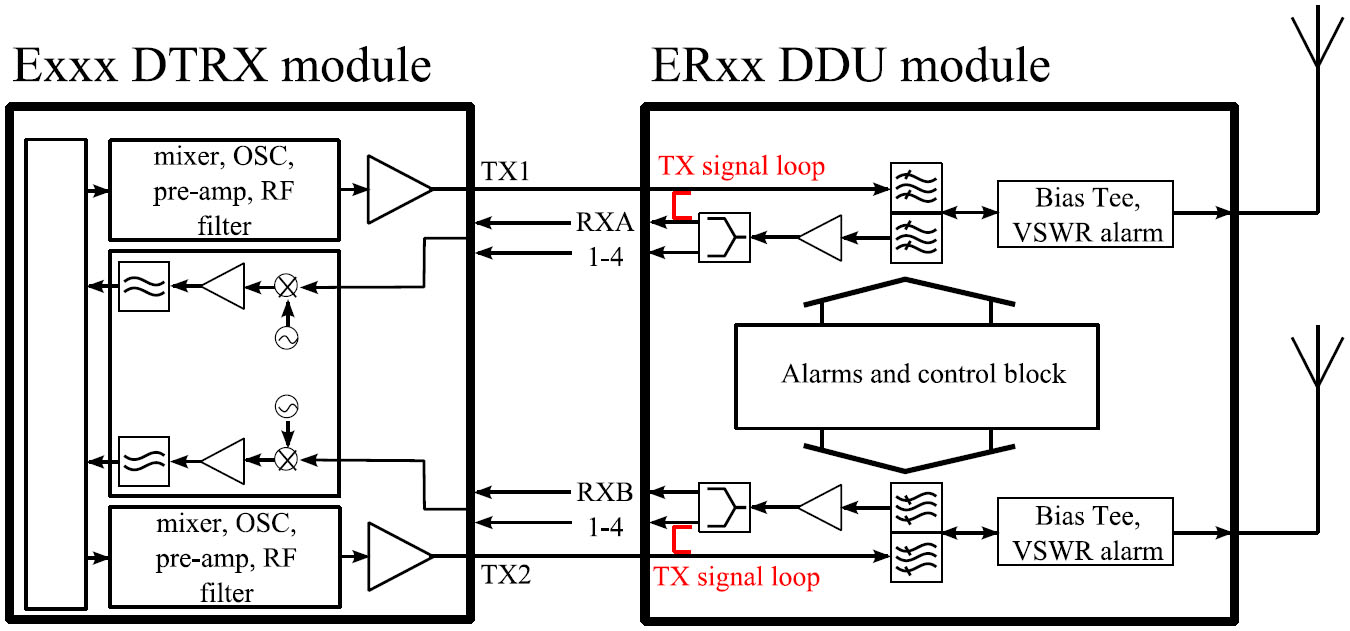
\includegraphics[width=\textwidth]{img/bs.jpg}
	\caption{Receiver under study.}
	\label{f:bs}
	\end{center}
	\vspace*{-12pt}
\end{figure}


\newpage
\section{Measurement steps}

In this section, used measurement configurations are presented for each measurement 
task. Measurements in question may be divided into two distinct categories: power 
measurements with a spectrum analyzer (SA) and two-port transmission measurements ($S_{21}$)
with a vector network analyzer (VNA). There were no significant differences between 
the planned setups and those used in the actual measurements. The following measuremeent 
specific subsections will elaborate.


\subsection{1~dB compression point}

To measure 1~dB compression point of a device, one needs a (manually) sweepable signal source 
and power detector. These may come separately or be incorporated in a single device. 
In both cases, the DDU module is connected the in between the source and the detector.
We used both approaches, and made two measurements with equal power levels.

For separate signal generation and detection, we used Rohde \& Schwarz SML03 signal 
generator and HP 8596E spectrum analyzer. The measurement setup is shown in Figures 
\ref{f:sg1} and \ref{f:sg2}. The setup where VNA is used is shown in Figures \ref{f:vna1} 
and \ref{f:vna2}. The attenuation caused by the two cables measured a cable at a time 
using VNA in a similar configuration. All equipment were calibrated before any measurements 
were carried out.

\begin{figure}[h!]
	\begin{center}
	\setlength{\unitlength}{1mm}
	\begin{picture}(142, 13)
		\linethickness{0.2mm}
		\put(0, 0.4){\framebox[34mm]{Signal generator}}
		\put(34, 1.4){\vector(1,0){20}}
		\put(54, 0.4){\framebox[28mm]{$\mathrm{ANT} \rightarrow \mathrm{RX}_1$}}
		\put(82, 1.4){\vector(1,0){20}}
		\put(102, 0.4){\framebox[40mm]{Sprectrum analyzer}}
		\put(68, 7){\makebox(0,0){DDU module}}
	\end{picture}
	\vspace*{\halfLine}
	\caption{Measurement setup used in the first measurement task.}
	\label{f:sg1}
	\end{center}
	\vspace*{-12pt}
\end{figure}

\begin{figure}[h!]
	\begin{center}
	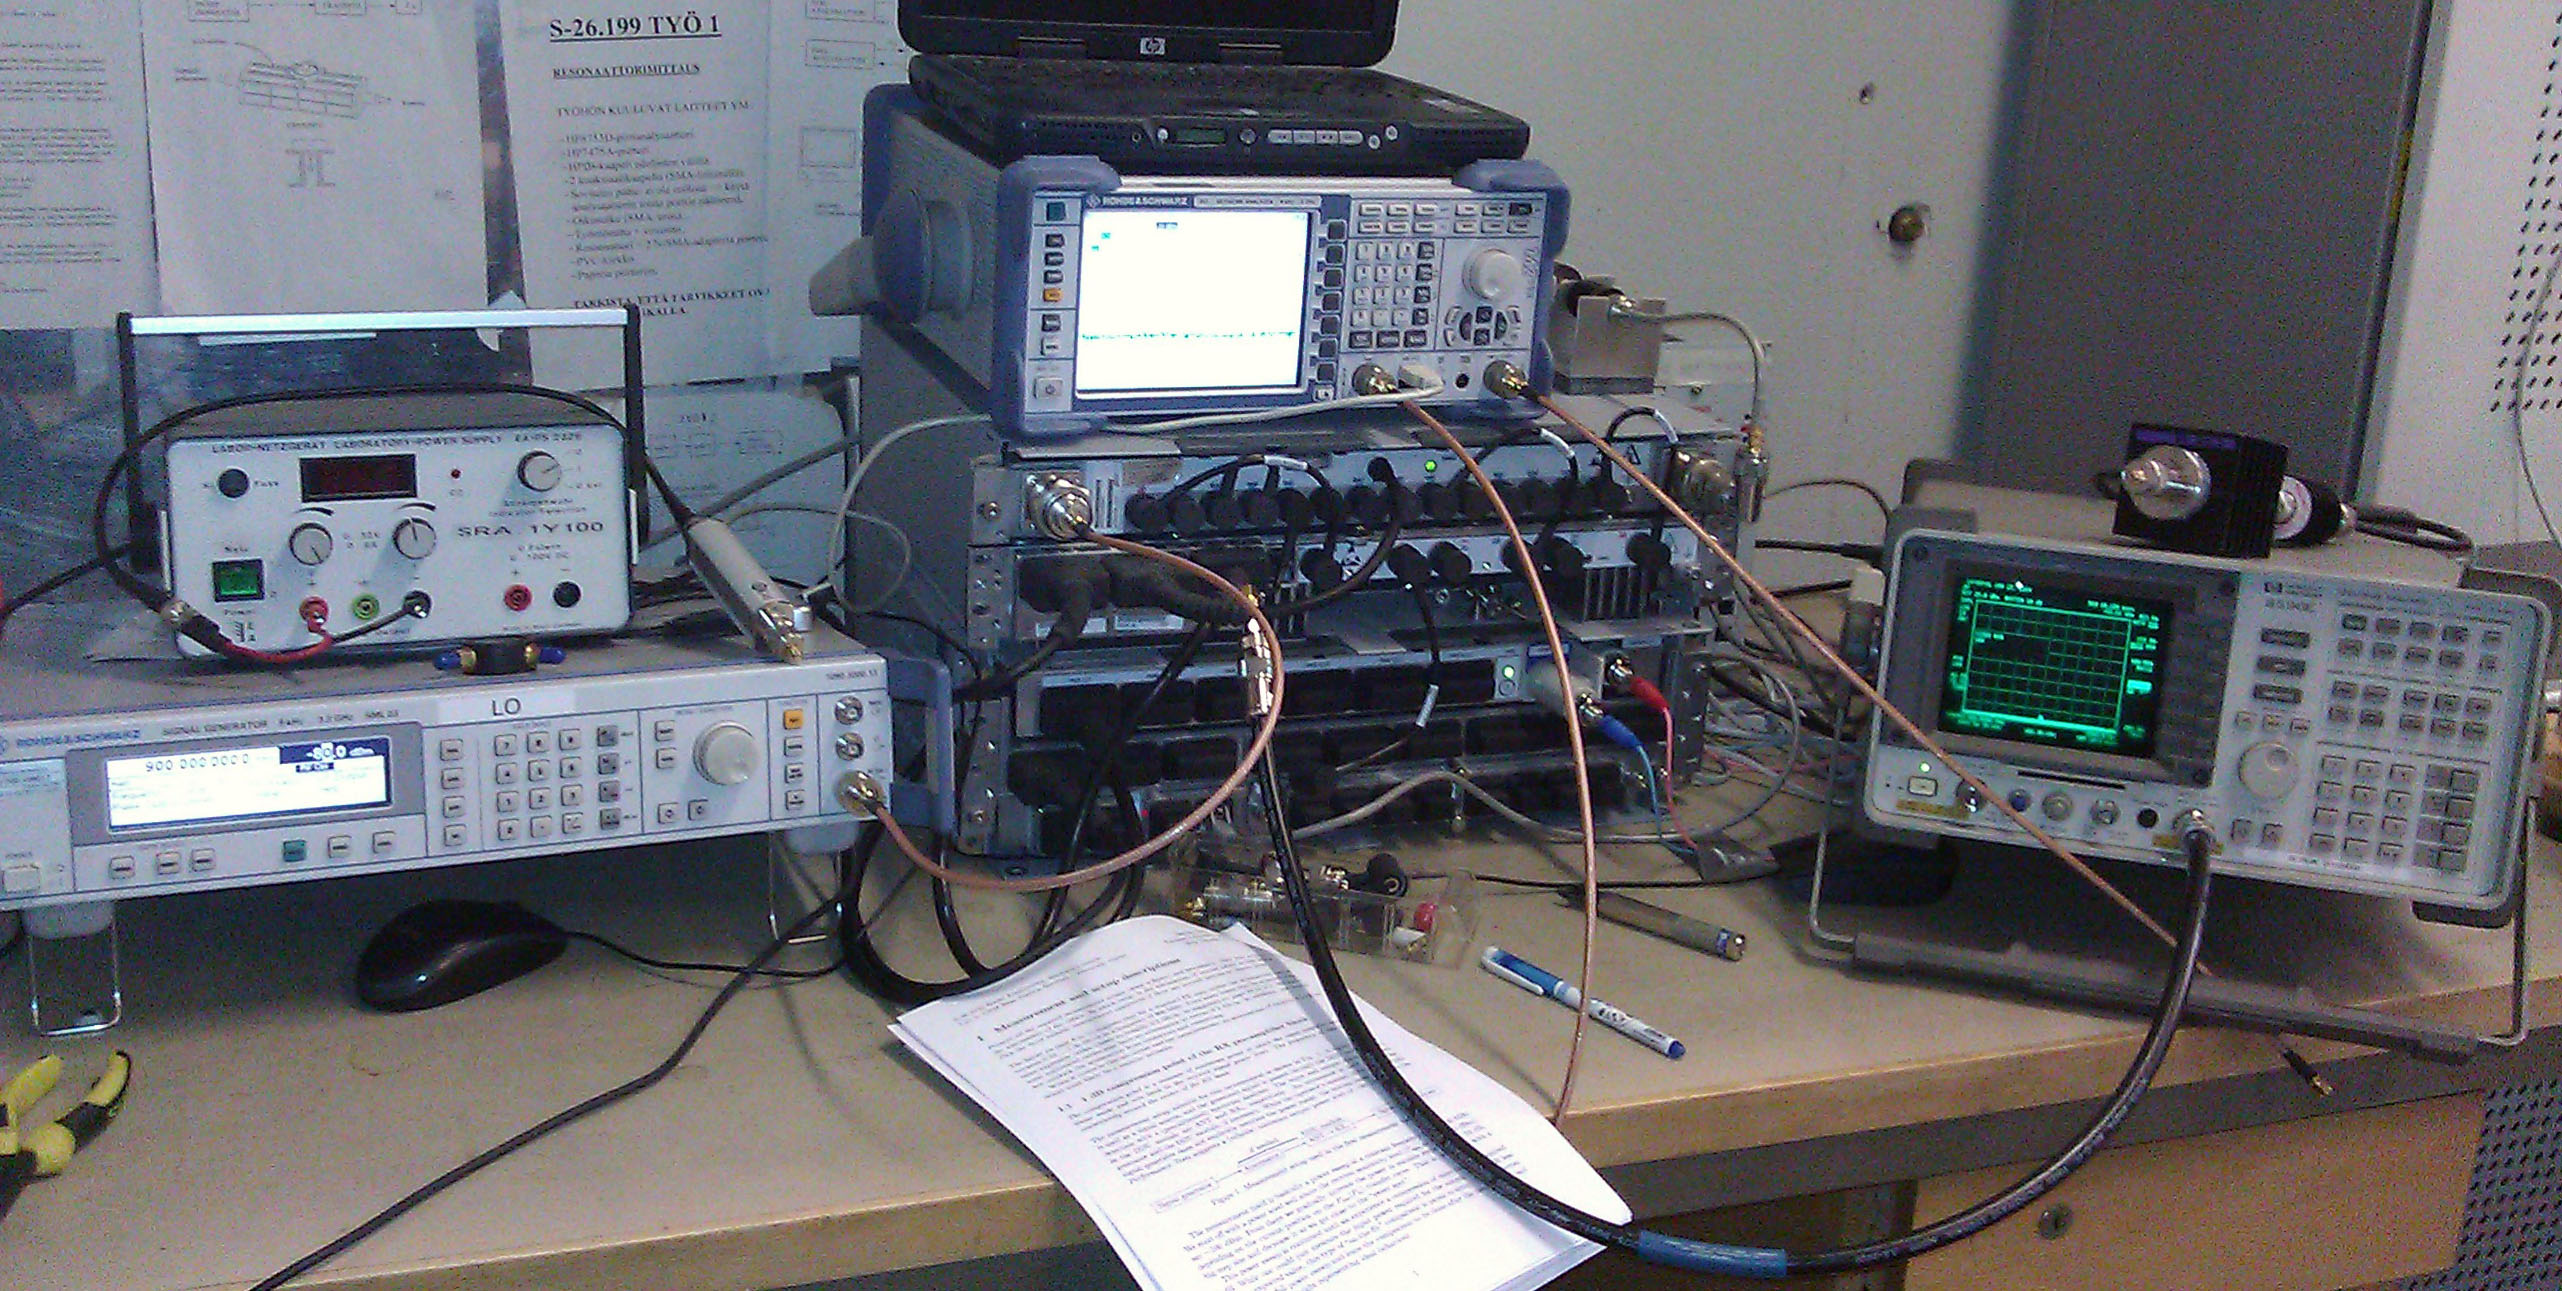
\includegraphics[width=0.75\textwidth]{img/sg-ddu-sa.jpg}
	\caption{Using a signal generator and spectrum analyzer to characterize the DDU module.}
	\label{f:sg2}
	\end{center}
	\vspace*{-12pt}
\end{figure}

\begin{figure}[h!]
	\begin{center}
	\setlength{\unitlength}{1mm}
	\begin{picture}(126, 10)
		\linethickness{0.2mm}
		\put(0, 0.4){\framebox[29mm]{VNA (Port 1)}}
		\put(29, 1.4){\vector(1,0){20}}
		\put(49, 0.4){\framebox[28mm]{$\mathrm{ANT} \rightarrow \mathrm{RX}_1$}}
		\put(77, 1.4){\vector(1,0){20}}
		\put(97, 0.4){\framebox[29mm]{VNA (Port 2)}}
		\put(63, 7){\makebox(0,0){DDU module}}
	\end{picture}
	\vspace*{\halfLine}
	\caption{VNA measurements connections}
	\label{f:vna1}
	\end{center}
	\vspace*{-12pt}
\end{figure}

\begin{figure}[h!]
	\begin{center}
	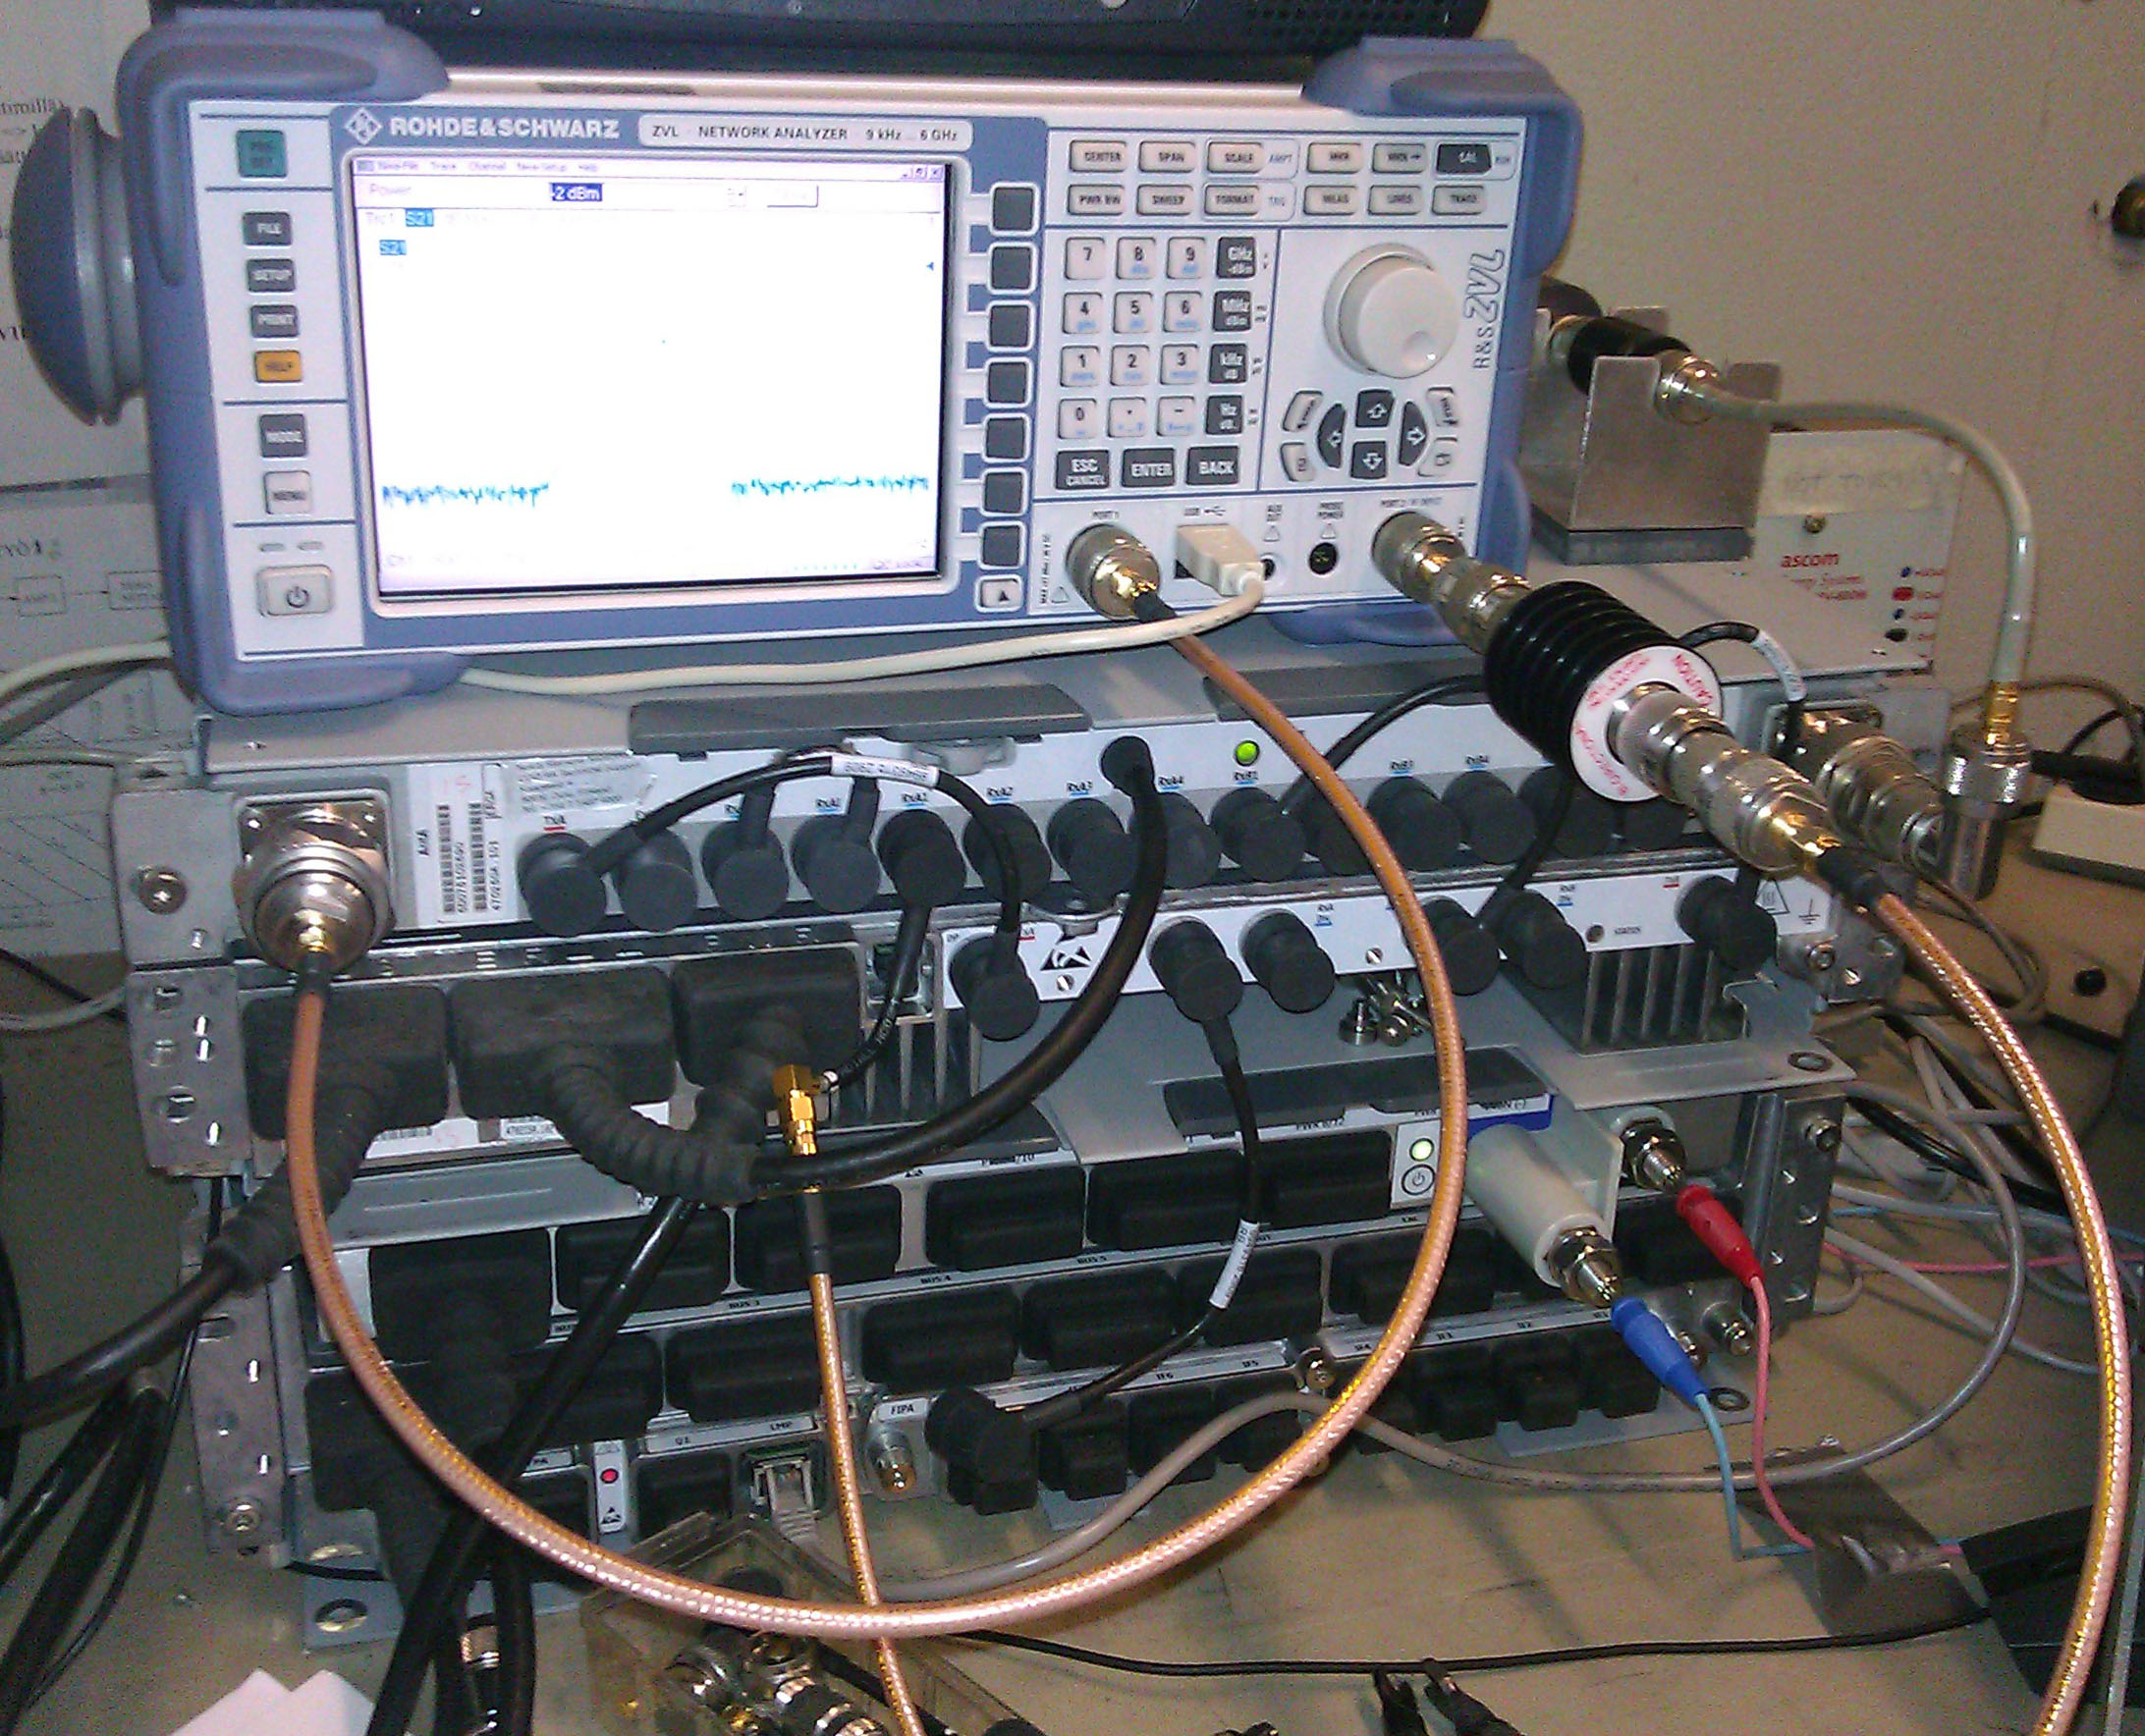
\includegraphics[width=0.75\textwidth]{img/vna-ddu-vna.jpg}
	\caption{Measuring the DDU module with the VNA.}
	\label{f:vna2}
	\end{center}
	\vspace*{-12pt}
\end{figure}




The measurement setup suitable for measuring measurement is shown in Fig. \ref{f:m1}. 
A signal generator is used as a signal source, and the generated signal is passed 
through the DDU module before detection with a (precalibrated) spectrum analyzer. 
The input and output connections used in the DDU module are ANT and RX$_1$, 
respectively. An attenuator is used between the generator and the DDU module, 
if necessary. While the operator's manual of the R\&S SML03 signal generator 
does not explicitly mention the power range, the testing range defined in the 
\textit{Performance Tests} suggests a (reliable) minimum output power level 
of $-80$~dBm.



The measurement itself is basically a power sweep at a constant frequency of 
$f = 900$ MHz. We start off with a power level well above the receiver sensitivity 
level ($P_\mathrm{min,\;BS} \approx -112.5$~dBm), say $-100$~dBm. From there we 
gradually increase the power in suitable steps of $0.1 \ldots 10$~dB, depending on 
the current position on the $P_\mathrm{out}(P_\mathrm{in})$ transfer curve. That 
is, we'll start with a big step size and decrease it as we get close to the 
``sweet spot''. 

This power sweep is continued until we experience a compression of more than the 
required 1 dB. While one could just measure the input power required for the output 
to be 1 dB less than the expected value, this type of ``on-the-fly'' comparison 
is prone to error. Thus it's better to measure a full power sweep and leave the 
comparison to be done after the measurement and against a fitted straight representing 
ideal behaviour.

Since we are dealing with a GSM receiver, we may use the same settings for the 
spectrum analyzer as we did in the first labs -- except for the averaging factor. 
They were as follows: an averaging factor of 500, zero span and 30~Hz video and 
resolution bandwidths. An averaing factor of 500 would make the measurement quite 
lengthy, especially if dense power ``grid'' is used. Averaging over 100 measurements 
will most likely be more than adequate. Depending on the 1~dB compression point, 
we might need to watch out for compression in the spectrum analyzer. This is taken 
care of by altering the input attenuation.

The effect of the cables and the attenuator may be measured using a VNA (could be used 
for the entire measurement aswell), or using the SA by making the whole measurement 
relative. In a relative measurement, the power is measured again when the DDU module 
is by-passed to account only for the cables and the possible attenuator. This also 
required to know the real input power. 


\subsection{Frequency response}

Wasn't this already covered in the first laboratory assignment as a part of the 
diplexer characterization? Fig. \ref{f:m2} presents the measurement setup used 
there. The DDU module is simply connected between the two ports of a precalibrated 
VNA; ANT and RX$_1$ connectors of the DDU module are connected to ports 1 and 2 of 
the VNA, respectively. In the VNA, measurement power shoud be as high as possible 
due the stop band-attenuation, yet simultaneously small enough not to cause 
compression in the pass-band (in neither the VNA nor in the pre-amp itself).

\begin{figure}[h!]
	\begin{center}
	\setlength{\unitlength}{1mm}
	\begin{picture}(126, 10)
		\linethickness{0.2mm}
		\put(0, 0.4){\framebox[29mm]{VNA (Port 1)}}
		\put(29, 1.4){\vector(1,0){20}}
		\put(49, 0.4){\framebox[28mm]{$\mathrm{ANT} \rightarrow \mathrm{RX}_1$}}
		\put(77, 1.4){\vector(1,0){20}}
		\put(97, 0.4){\framebox[29mm]{VNA (Port 2)}}
		\put(63, 7){\makebox(0,0){DDU module}}
	\end{picture}
	\vspace*{\halfLine}
	\caption{Measurement setup used when determining the gain of the pre-amplifier block.}
	\label{f:m2}
	\end{center}
	\vspace*{-12pt}
\end{figure}

The following figure (Fig. \ref{f:r1}) shows the results obtained in the first lab works 
with a transmit power of $-20$ dBm in the VNA (using the B-half of the BS and connecting 
the ports vice versa). In the figure, in addition to GSM RX and TX bands (in red), both 
3~dB (in blue) and noise (in green) bandwidth of the pre-amp block are visualized. This 
noise bandwidth visualization is somewhat questionable as it's a purely theoretical concept, 
but is nevertheless shown for scale. The shown noise bandwidth is found using a numerical 
approximation with $|S_{12}|$ of the formula given in the lecture supplement handout:

\begin{equation}
B_\mathrm{n} = \frac{1}{G_\mathrm{T,\;max}} \int_0^\infty G_\mathrm{T}(f) \, df.
\end{equation}

The noise bandwidth shown is less than the actual band since we cannot use infinite frequency 
range. Frequency range of $850 \ldots 1000$~MHz with $|S_{12}|_\mathrm{max} = 24.4$~dB 
was used instead. The obtained value (38.1~MHz) is roughly 6~\% shy of the 3~dB bandwidth 
(40.6~MHz), as one might expect. The 3~dB bandwidth may thus be used to avoid being 
overly optimistic.

\begin{figure}[h!]
	\begin{center}
	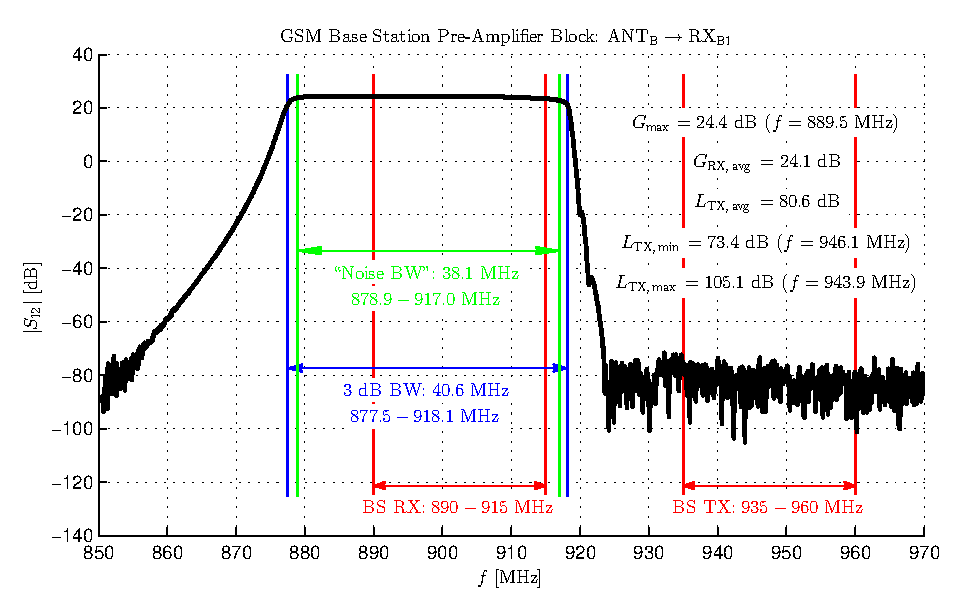
\epsfig{file=img/s12.eps, width=\textwidth}
	\caption{Results from the diplexer characterization.}
	\label{f:r1}
	\end{center}
	\vspace*{-12pt}
\end{figure}

In the graphical approximation method we need to investigate the effect of frequency 
roll-off speed. From Fig. \ref{f:r1} the transition bands are approx. 30~MHz (3.4 \%) 
and 5~MHz (0.55 \%) for lower and upper bands, respectively. During this transition, 
the $S_12$ drops roughly 100~dB from $+20$~dB to $-80$~dB. This corresponds to a slope 
of $3.3$~dB/MHz (29~dB/\%) and $-20$~dB/MHz ($-180$~dB/\%), respectively. The effect of 
such steep slopes are neglectable, and thus the 3~dB bandwidth may be used as the noise 
bandwidth.

If a VNA is not available as the instructions suggest, the task is quite laborious and 
absurd, just to be honest. Nevertheless, the procedure is listed here for completeness. 
We would need to simulate the VNA function manually using a signal generator and a power 
meter or a signal analyzer, leading to a setup like the one shown in Fig. \ref{f:m1}. The
output power is kept constant while frequency is swept over the range, taking notes on the 
relative power levels observed in the detector.

\begin{comment} % As an example
\begin{table}[!h]
	\begin{center}
	\caption{Two-ports measured with the VNA.}
	\label{tbl:2p}
	\renewcommand*{\arraystretch}{1.2}
	\begin{tabular}{ll}
	\textbf{Measurement} & \textbf{Two-port} \\
	\hline
	3.1 $-$ 3.3		& SMA-cable $+$ attenuator chain $+$ N-cable $+$ required adapters \\
	3.4 (a)			& $\mathrm{TX_B \rightarrow ANT_B}$ 	\\
	3.4 (b)			& $\mathrm{TX_B \rightarrow RX_{B1}}$ 	\\
	3.4 (c)			& $\mathrm{ANT_B \rightarrow RX_{B1}}$
	\end{tabular}
	\end{center}
	\vspace*{-12pt}
\end{table}
\end{comment}


\subsection{Noise temperature}

ENR = 21.48 dB

In the third measurement task, we'll use a setup shown in Fig. \ref{f:m3}. 
A DC-voltage source is connected to a noise diode connected directly to the 
ANT-input in the pre-amplifier block. This direct connection is desirable as 
attenuation changes the noise temperature. The signal is led from the RX$_1$ 
output to a spectrum analyzer. An LNA may be needed in between the DDU output 
and the spectrum analyzer, as the spectrum analyzer might not be sensitive 
enough for the cold noise source.

\begin{figure}[h!]
	\begin{center}
	\setlength{\unitlength}{1mm}
	\begin{picture}(163, 13)
		\linethickness{0.2mm}
		\put(0, 0.4){\framebox[10mm]{$V_\mathrm{DC}$}}
		\put(10, 1.4){\vector(1,0){12}}
		\put(22, 0){\framebox[25mm]{Noise diode}}
		\put(47, 1.4){\vector(1,0){12}}
		\put(59, 0.4){\framebox[28mm]{$\mathrm{ANT} \rightarrow \mathrm{RX}_1$}}
		\put(87, 1.4){\vector(1,0){12}}
		\put(99, 0.4){\framebox[12mm]{LNA}}
		\put(111, 1.4){\vector(1,0){12}}
		\put(123, 0.4){\framebox[40mm]{Sprectrum analyzer}}
		\put(5, 7){\makebox(0,0){0/28 V}}
		\put(73, 7){\makebox(0,0){DDU module}}
	\end{picture}
	\vspace*{\halfLine}
	\caption{Noise temperature measurement setup}
	\label{f:m3}
	\end{center}
	\vspace*{-12pt}
\end{figure}

%In room temperature, a matched load (an approximation in this case) outputs a noise power 
%of $-159$ dBm for a 30 Hz band. With a maximum gain of 24.4~dB and a total noise figure 
%of 3.9~dB, the expected noise level is around $-131$~dBm. This value is considerably 
%lower than the given sensitivity of the SA: $P_\mathrm{SA,\;min} < -125$~dBm when 
%$B_\mathrm{res.} = 30$~Hz. LNA could be used to boost the signal to a more appropriate 
%level as it's effect on the noise temperature could be compensated using the Friis' 
%noise formula.

The measurement itself is carried out measuring two power levels required in the 
Y-pa\-ram\-e\-ter; when the DC-voltage is off/shorted (``cold'') and on (``hot''). As 
for the SA settings, we are measuring noise at a single frequency (using zero-span): 
a very weak, random signal. Thus, input attenuator should be disabled, and minimum 
resolution bandwith used. A large averaging factor, say a thousand, is also beneficial. 
The measurement may take a few minutes, and it's OK; there are only two measurements 
to be made.

\begin{figure}[h!]
	\begin{center}
	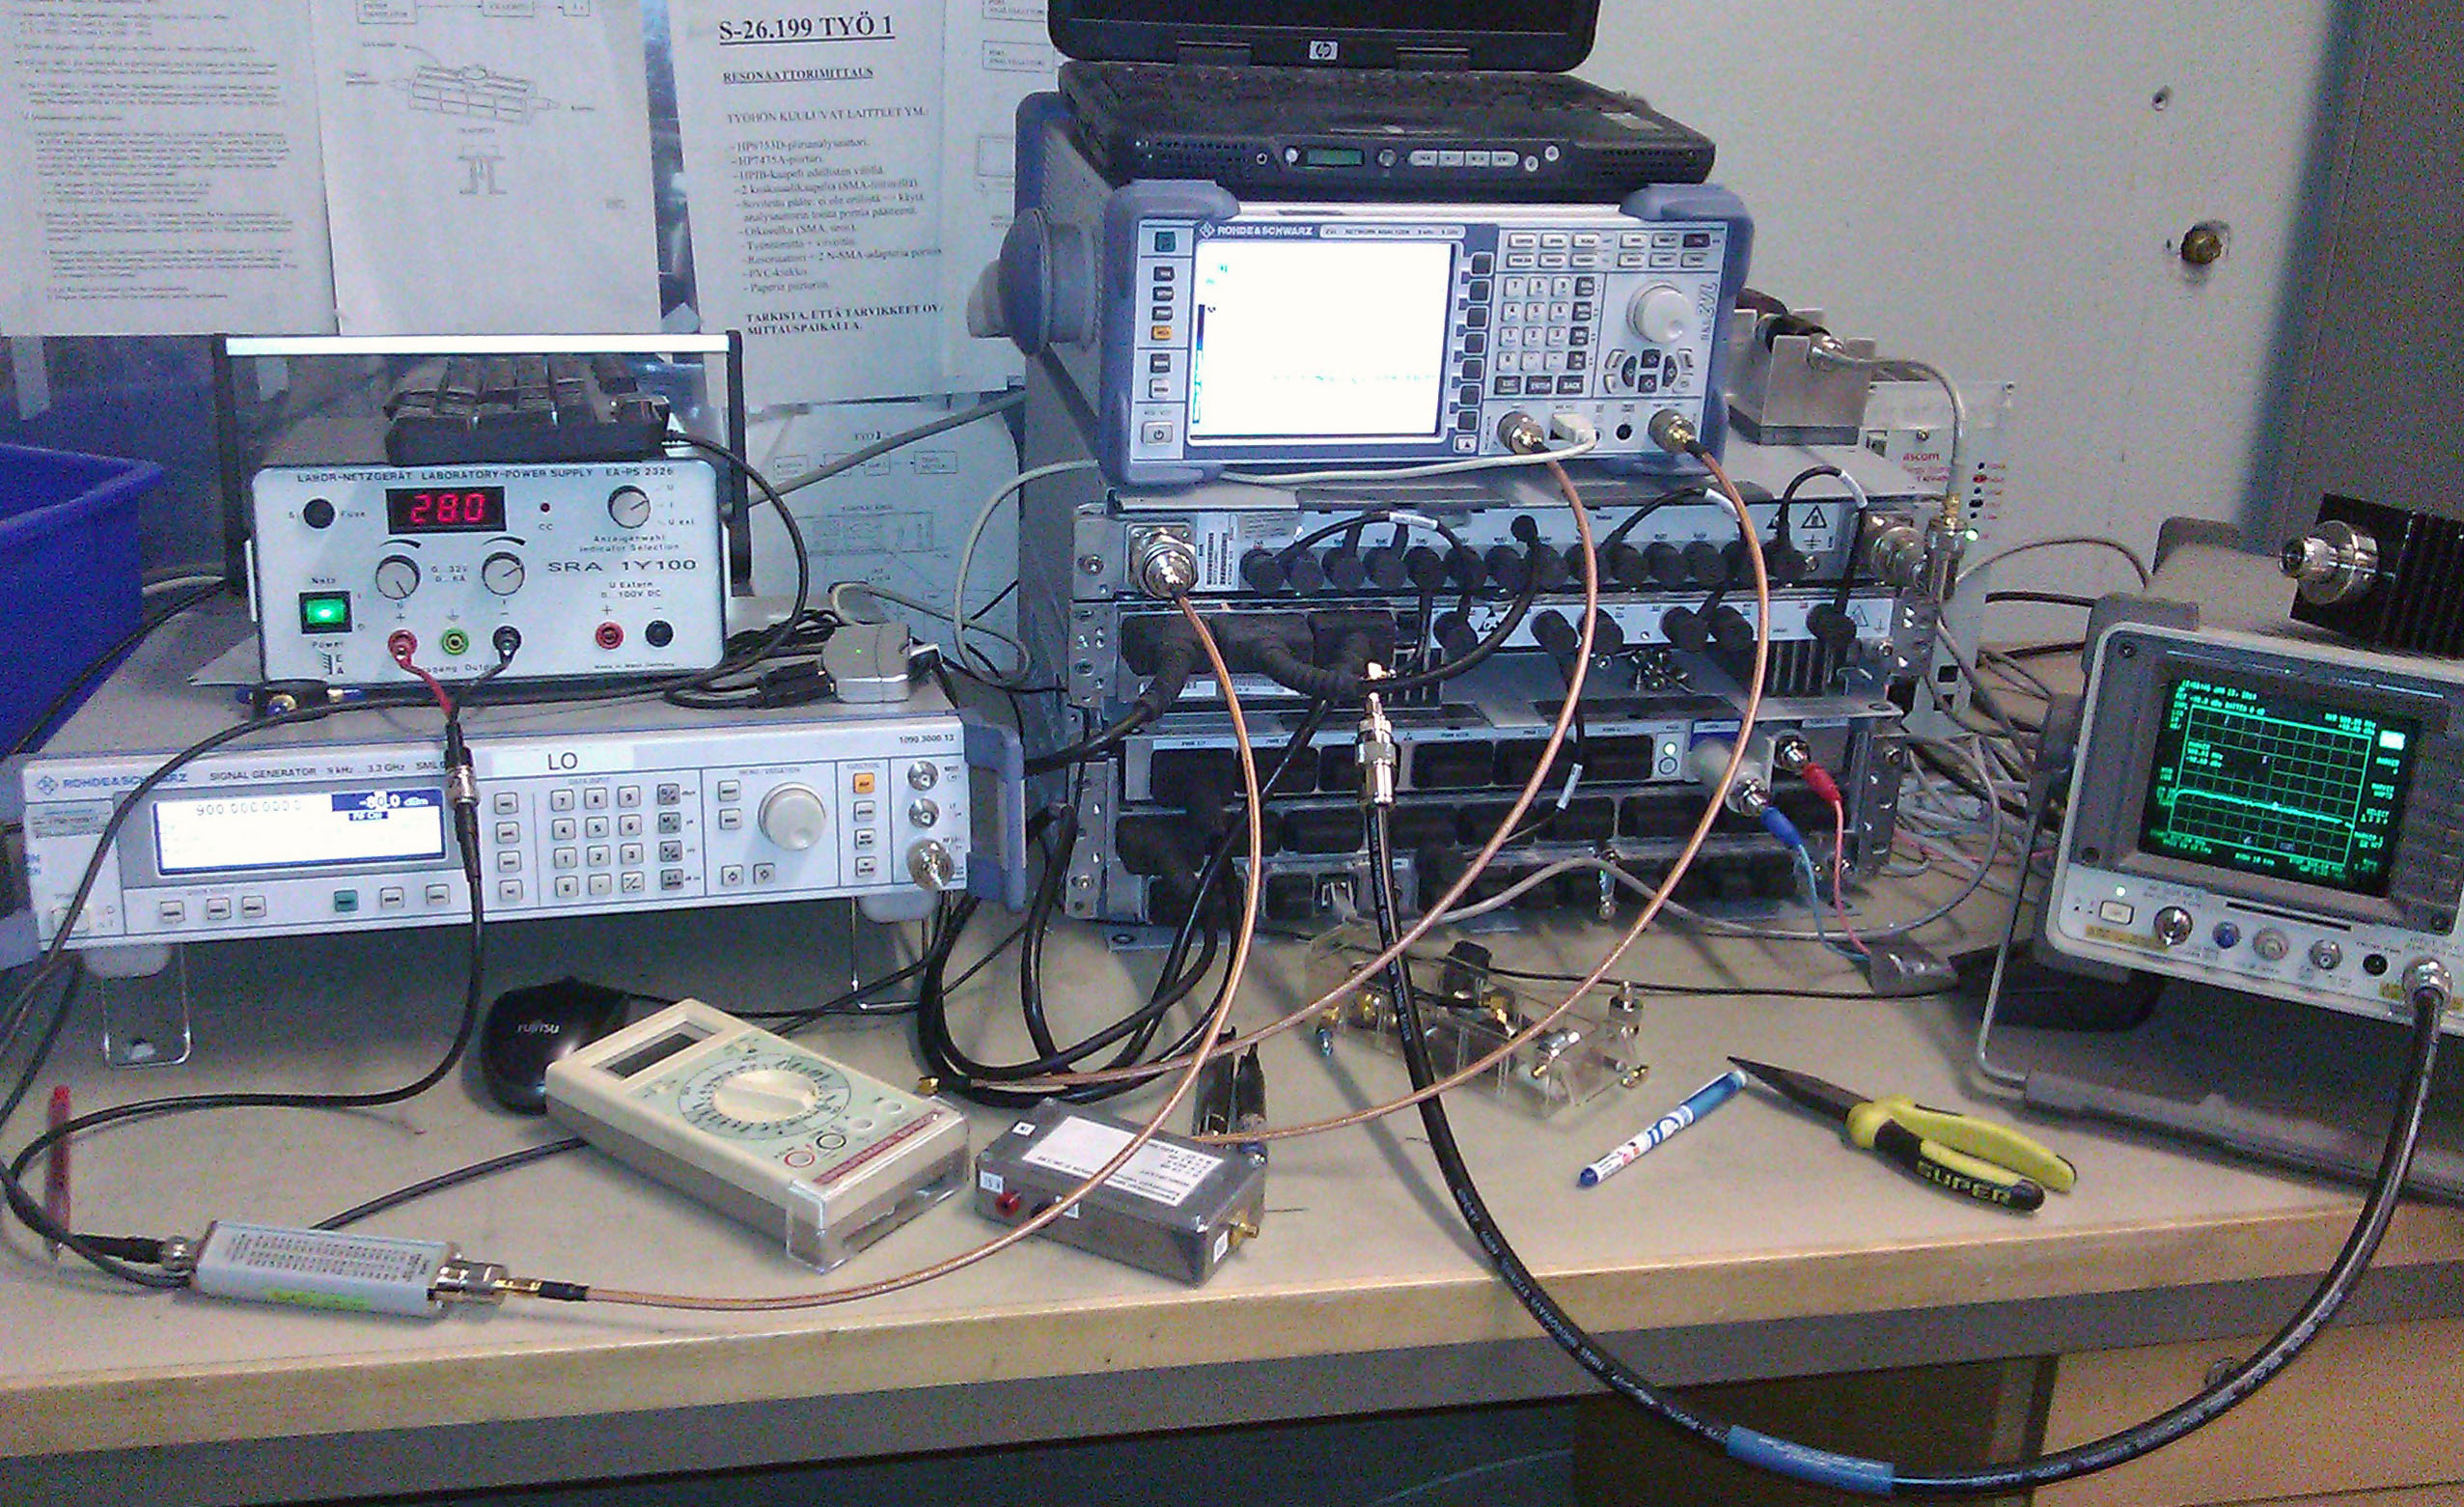
\includegraphics[width=0.75\textwidth]{img/nd-ddu-sa.jpg}
	\caption{Receiver under study.}
	\label{f:nd}
	\end{center}
	\vspace*{-12pt}
\end{figure}

\subsection{Sensitivity}

In the sensitivity measurement, we're trying to measure the minimum input power at 
ANT input that results in a detectable signal above the noise floor in the ouput 
of the DDU module. For this, a measurement setup identical to the one used in the 
first task may be used, as is shown in the following figure (Fig \ref{f:m4}). This 
time though it's more than likely that an attenuator is required.

\begin{figure}[h!]
	\begin{center}
	\setlength{\unitlength}{1mm}
	\begin{picture}(142, 13)
		\linethickness{0.2mm}
		\put(0, 0.4){\framebox[34mm]{Signal generator}}
		\put(34, 1.4){\vector(1,0){20}}
		\put(54, 0.4){\framebox[28mm]{$\mathrm{ANT} \rightarrow \mathrm{RX}_1$}}
		\put(82, 1.4){\vector(1,0){20}}
		\put(102, 0.4){\framebox[40mm]{Sprectrum analyzer}}
		\put(68, 7){\makebox(0,0){DDU module}}
	\end{picture}
	\vspace*{\halfLine}
	\caption{Measurement setup used in the sensitivity measurement.}
	\label{f:m4}
	\end{center}
	\vspace*{-12pt}
\end{figure}

The measurement starts by measuring the noise floor at 900~MHz without any signal 
we're hoping to detect. That is, the RF power is switched off at the generator. 
Then we turn on an input signal that's some dBs sensitivity of $-112.5$~dBm. We 
gradually increase the power until the signal-to-noise ratio is no less than the 
10~dB required by the standard. One could also measure the power required to beat 
the noise just barely, and add the SNR later on if  $P_\mathrm{out}(P_\mathrm{in})$ 
relation is assumed to be ideal.

Since it's a GSM system, we use the measurement settings as they are defined in 
the standard. They are as follows: an averaging factor of 500, zero span and 30~Hz 
video and resolution bandwidths. As the spectrum analyzer input power is expected 
to be less than $-80$~dBm ($P_\mathrm{SA} \approx P_\mathrm{DDU,\;min} + G_\mathrm{DDU} = -112.5 \mathrm{\;dBm} + 24.4 \mathrm{\;dB}= -88.1 \mathrm{\;dBm}$), 
it's best to disable the input attenuator.


\newpage
\section{Results}

TODO: Huy and Sampo (general results and intro to more specific results)


\subsection{1~dB compression point}

\begin{figure}
\centering
\subcaptionbox{$P_\mathrm{out}(P_\mathrm{in})$ using SG and SA}{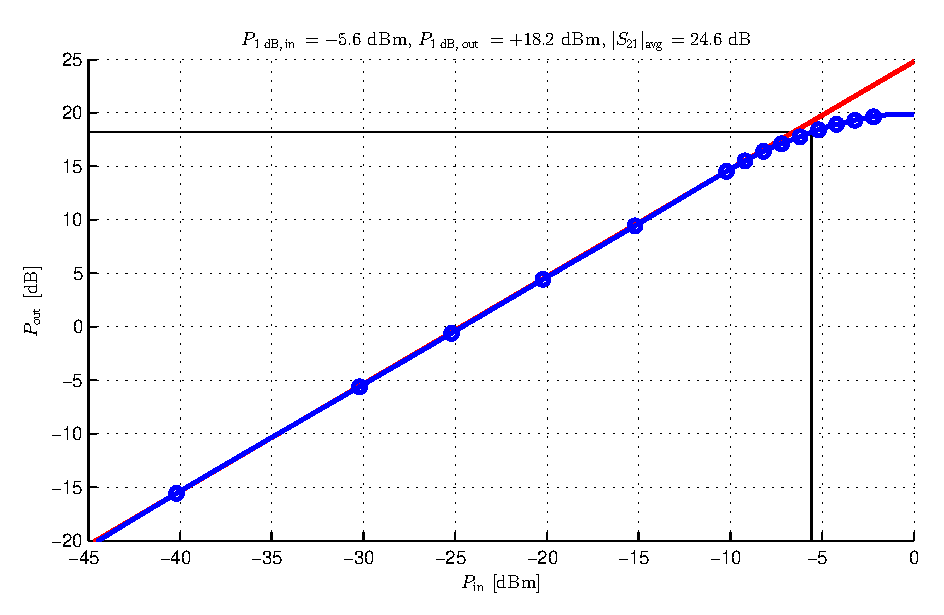
\epsfig{file=img/PoutPin1.eps, width=0.45\textwidth}}
\subcaptionbox{$P_\mathrm{out}(P_\mathrm{in})$ using VNA}{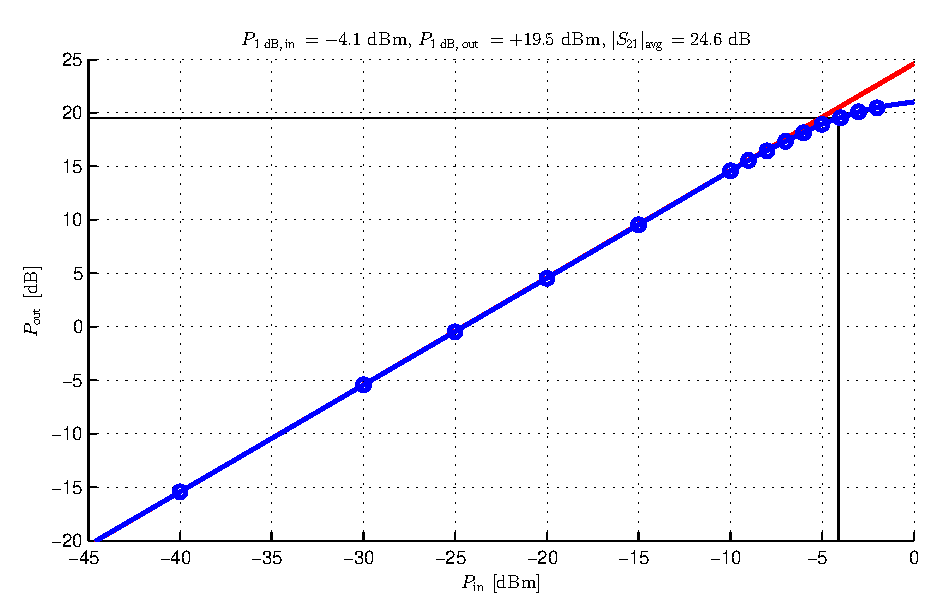
\epsfig{file=img/PoutPin2.eps, width=0.45\textwidth}}
\subcaptionbox{$G(P_\mathrm{in})$ using SG and SA}{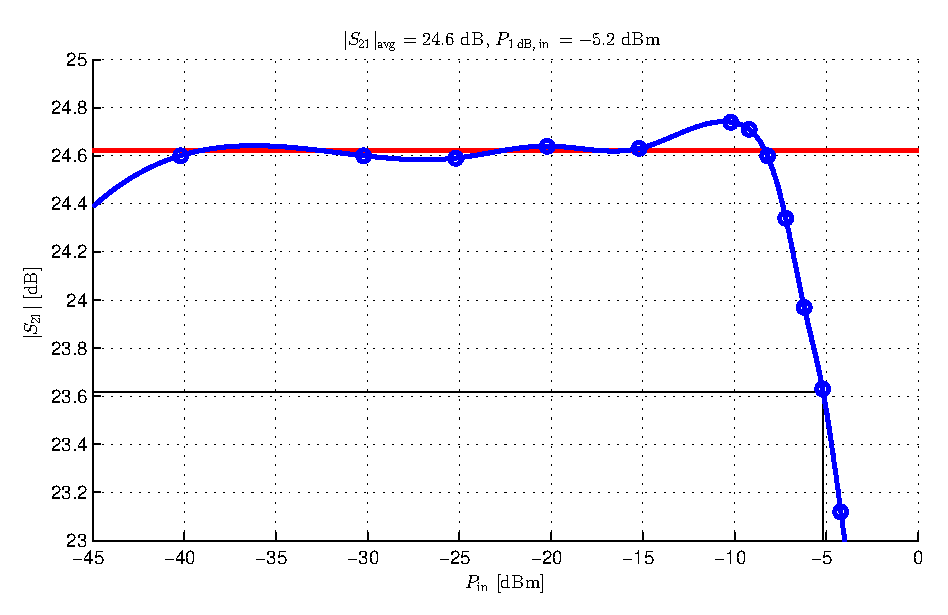
\epsfig{file=img/GPin1.eps, width=0.45\textwidth}}
\subcaptionbox{$G(P_\mathrm{in})$ using VNA}{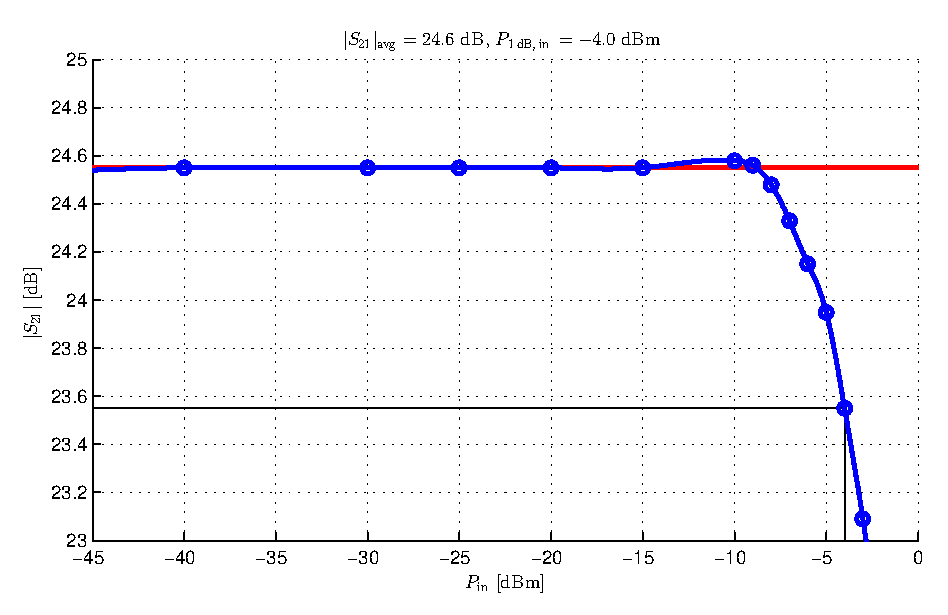
\epsfig{file=img/GPin2.eps, width=0.45\textwidth}}
\subcaptionbox{$G(P_\mathrm{out})$ using SG and SA}{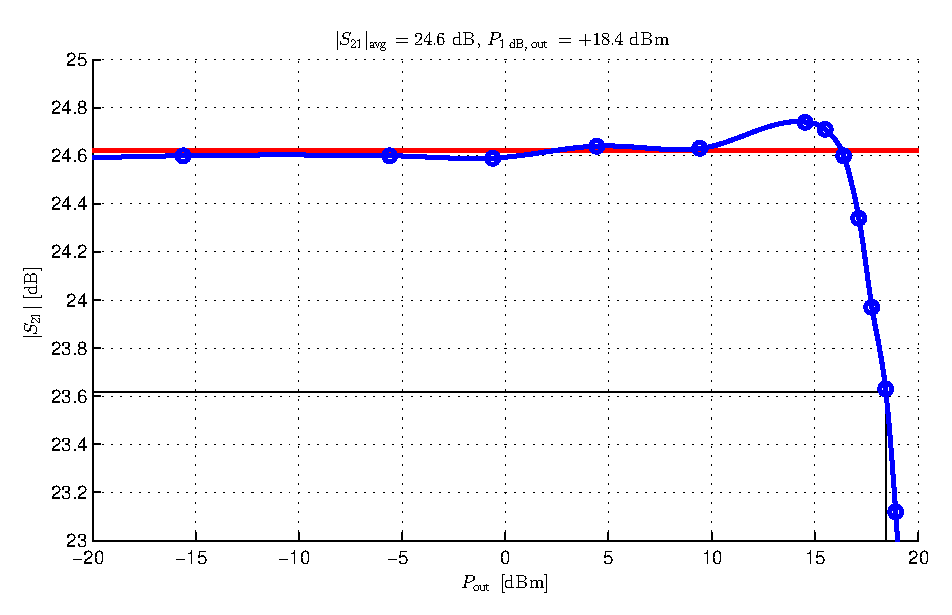
\epsfig{file=img/GPout1.eps, width=0.45\textwidth}}
\subcaptionbox{$G(P_\mathrm{out})$ using VNA}{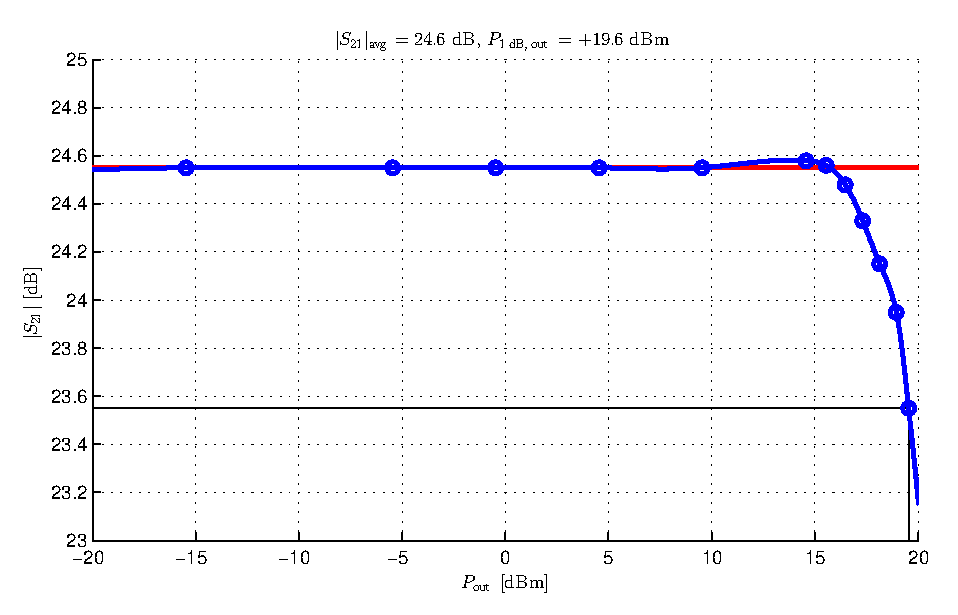
\epsfig{file=img/GPout2.eps, width=0.45\textwidth}}
\caption{Results from the 1~dB compression point measurements. Ideal behaviour is shown with red straights, measuremets with blue markers and spline inter-/extrapolant in blue.}\label{f:1dB}
\end{figure}


\subsection{Frequency response}

\begin{figure}[h!]
	\begin{center}
	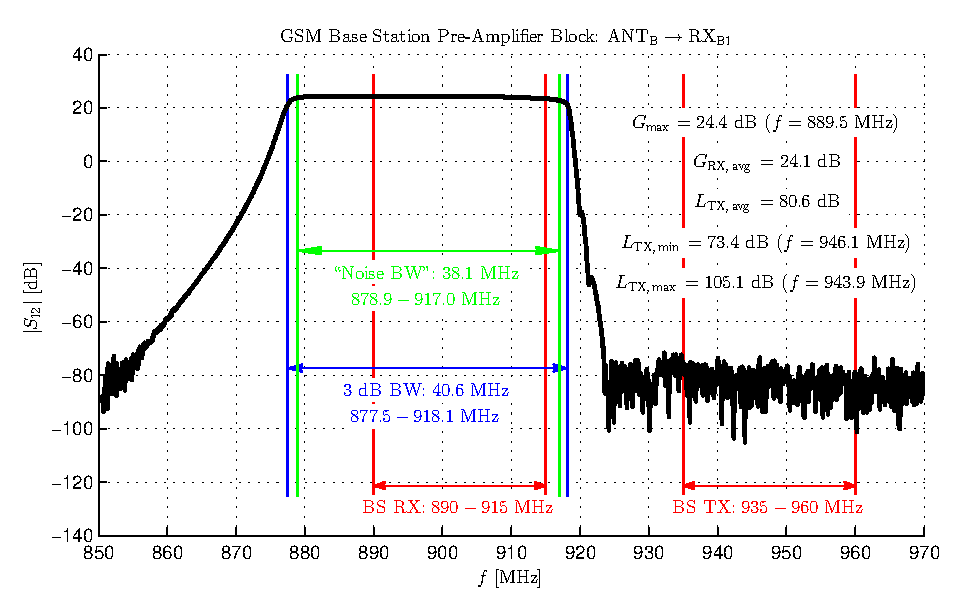
\epsfig{file=img/s12.eps, width=\textwidth}
	\caption{Results from the diplexer characterization.}
	\label{f:dpx}
	\end{center}
	\vspace*{-12pt}
\end{figure}


\subsection{Noise Temperature}

TODO: Huy and Sampo


\subsection{Sensitivity}

TODO: Huy and Sampo


\subsection{Dynamic range}

TODO: Huy and Sampo


\newpage
\section{Error estimates}

TODO: Huy and Sampo (make additions, corrections, change the style to avoid excess 
repetition etc.)

In this section, error estimates for the two types of measurements are presented.
The values presented here are only rough estimates based on literature (with more 
or less general cases) and their soundness in this case is somewhat questionable. 
In this section, we do not take human errors (see previous section) into account. 
It is just stated that systematic errors arising from the cables and connections 
are possible in measurement all measurements. Thus they are valid only for 
``correct'' measurements, and are more of the ``provided for completeness'' 
nature. Probabilities are not given due to the nature/basis of the estimation.


\subsection{Spectrum analyzer}

Each of the components inside the spectrum analyzer contributes to the total uncertainty, 
depending for example on the signal frequencies, amplitudes, and measurement settings. 
The Agilent (former HP, manufacturer of the used SA) has made available a document that 
specifies the different error sources, giving also rough estimates for some spectrum 
analyzers. According to the document \cite{sa}, the error estimates vary broadly among 
different analyzer models, giving worst case uncertainties exceeding $\pm 6$ dB. On the 
other hand, the document gives also representative values of amplitude uncertainties, 
which in our case yields about $\pm 1$ dB.

The second error source for the spectrum analyzer is the power marker reading. In 
each of the tasks, the spectrum analyzer was set to average 500 measurement points, 
which should average out most of the random errors. However, reading the power marker 
in the screen, there was a noticeable fluctuation in the shown power value. Based on the 
experience obtained during the measurements, the power marker error is estimated to be 
approximately $\pm 0.5$ dB.

In conclusion, the error estimates that can be taken into account numerically are 
the manufacturers representative value of approx. $\pm 1$ dB, and the power marker 
fluctuation of roughly $\pm 0.5$ dB. These uncorrelated errors may be summed to 
achieve the total uncertainty of the SA measurements of approx. $\pm 1.5$ dB. 

There is also the question of calibrating the spectrum analyzer properly with 
the time interval defined by the manufacturer. Agilent suggests to have the spectrum 
analyzer calibrated thoroughly once in a year, and quick-calibrated if there are 
changes operating environment \cite{sa2}. If the spectrum analyzer used in the 
measurements is not calibrated correctly, it is possible that the measurements are 
not reliable. In this case, the calibration is the most important error source, and 
the device should be calibrated correctly before estimating any other errors.


\subsection{Vector network analyzer}

For the VNA, different error sources and ways to cope with them are listed in the 
lecture slides discussing VNA measurements. The different sources are noise, 
cabling/connector repeatability, directivity, isolation, mismatch and environment 
induced drift. 

Noise and cabling/connector repeatability are random errors, which can be averaged 
out. In our case, only the noise was averaged, since we did not touch the cabling. 
Systematic errors arising directivity, isolation, and mismatch in this task were
for the most part neglected with a calibration. Before conducting measurements, 
the VNA is always calibrated using a standard calibration module. The calibration 
moves the reference planes to the connectors of the test cables, and somewhat 
cancels the systematic errors from the connectors and cables used in a specific 
measurement. Finally, the environment induced drift is not relevant, since the 
measurement was done inside a short time interval.

Rohde \& Schwarz provides specifications that describe the measurement uncertainty 
of the VNA in question in different frequency bands. For transmission measurements 
in the frequency range of 50 MHz to 3 GHz, accuracy for signal powers of $-50 \ldots 0$ 
dB is better than $0.2$ dB ($0.3$ dB for powers of $-50 \ldots {-70}$ dB) with 0 dBm 
transmit power. \cite{vna} The reader should note that these ranges was exceeded 
from both ends during the measurements (the measurement power range was roughly 
$-100 \ldots {+4}$ dBm). 

In conclusion, two things are assumed. First, calibration is assumed to cancel the 
systematic errors arising from cables and connectors. Second, random errors are 
cancelled with averaging. The manufacturer provides error estimates for the device 
itself, giving an error estimate of under $0.3$ dB that is mostly applicable in 
our case. The topics discussed in the last paragraph of the last subsection apply 
here to some extent to here as well.


\subsection{Noise diode}

See lecture handout supplement.


\newpage
\section{Conclusions}

TODO: Huy and Sampo


\newpage
\section{Feedback}

TODO: Huy and Sampo (not all devices are listed in the instructions sheet, learning from feedback)


\newpage
\begin{thebibliography}{9}%\itemsep 7pt\parskip -5pt 

\bibitem{lab2} C.\ Icheln, S.\ Khanal, 
	\textit{GSM Receiver laboratory assignment instructions},
	S-26.3120 Laboratory course in Radio Engineering course material.
	
\bibitem{} C.\ Icheln (edited), 
	\textit{Lecture supplement handout},
	S-26.3120 Laboratory course in Radio Engineering course material.

\bibitem{sa} Agilent, Spectrum Analysis Basics, Application Note 150. 
	Available online at \url{http://cp.literature.agilent.com/litweb/pdf/5952-0292.pdf} 
	[Retrieved: Jan 2nd, 2014].
	
\bibitem{sa2} Agilent, 8590 Series Analyzers Calibration Guide.
	Available online at \url{http://cp.literature.agilent.com/litweb/pdf/08594-90106.pdf}
	[Retrieved: Jan 2nd, 2014].
	
\bibitem{vna} R\&S ZVL Vector Network Analyzer Specifications, 
	Version 06.00, Dec 2008. 
	Available online at \url{http://www.upc.edu/pct/documents_equipament/d_160_id-655-2.pdf} 
	[Retrieved: Jan 2nd, 2014].


%\bibitem{pozar} D.\ M.\ Pozar, 
%	\textit{Microwave Engineering}, 
%	J.\ Wiley \& Sons, 4th Edition, 2012. 
%	ISBN: 978-0-470-63155-3.
	
%\bibitem{gains} J.\ C.\ Logan, J.\ W.\ Rockway, 
%	``Dipole and Monopole Antenna Gain and Effective Area for Communication Formulas.''
%	Available online at \url{www.dtic.mil/cgi-bin/GetTRDoc?AD=ADA332891}
%	[Retrieved: November 25, 2013].

%\bibitem{parts} M.\ Steer, 
%	\textit{Microwave and RF Design -- A Systems Approach}, 
%	SciTech Publishing, 2010. 
%	ISBN: 978-1-891-12188-3.
	
%\bibitem{iet} R.\ J.\ Collier, A.\ D.\ Skinner (editors), 
%	\textit{Microwave Measurements}, 
%	The Institution of Engineering and Technology, 3rd Edition, 2007. 
%	ISBN: 978-0-86341-735-1.

\end{thebibliography}

\end{document}
